\section{Basics about Data Representation}
\label{sec:basic}
\begin{frame}<beamer>
    \frametitle{Outline}
    \tableofcontents[currentsection]
\end{frame}


\begin{frame}
\frametitle{Everything is binary code in computer (1)}
	\begin{itemize}
		\item {Everything in computer is in \textbf{binary} form}
		\item {Data: integers, real numbers and strings}
		\item {Instructions}
		\item {Addresses: sequential numbers for the memory cells}
	\end{itemize}
	\begin{itemize}
		\item {It is therefore necessary to know how the binary code is produced}
		\item {In addition, for convenience}
		\item {\textbf{Octal} and \textbf{Hexadecimal} numbers are also used for display}
	\end{itemize}
\end{frame}

\begin{frame}{Everything is binary code in computer (2)}
	\begin{figure}
			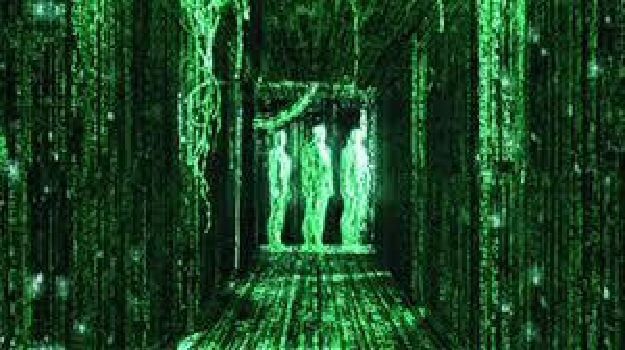
\includegraphics[width=0.6\linewidth]{figs/matrix.pdf}
	\end{figure}
	\begin{itemize}
		\item {Anyone watched this movie?}
	\end{itemize}
\end{frame}

\begin{frame}
\frametitle{Decimal to Binary, Octal and Hexadecimal (1)}
	\begin{figure}
		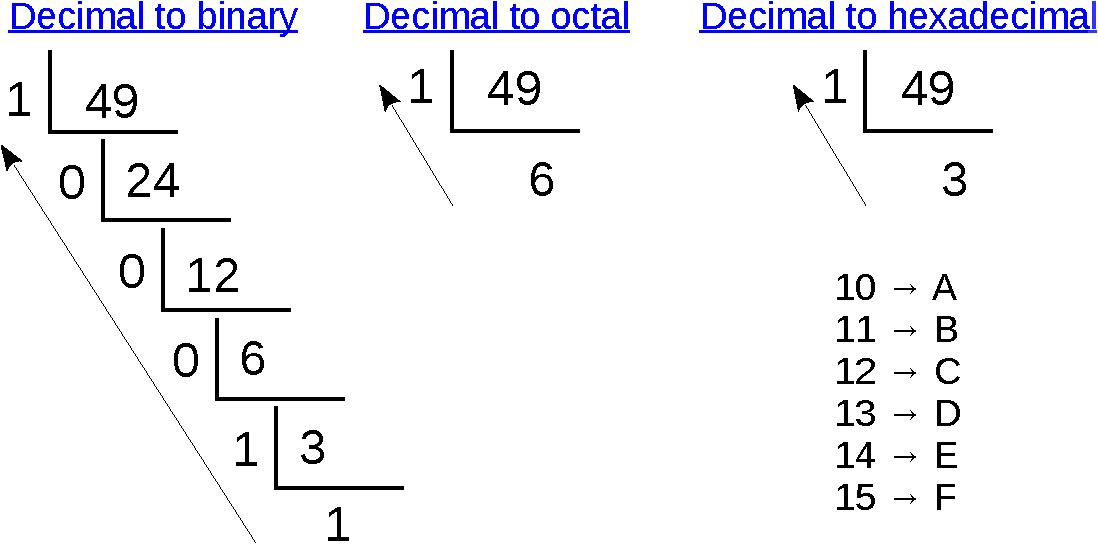
\includegraphics[width=0.75\linewidth]{figs/d2b.pdf}
	\end{figure}
	\begin{itemize}
		\item {Binary code: $110001_{(2)}$}
		\item {Octal code: $61_{(8)}$}
		\item {Hexadecimal code: $31_{(16)}$}
		\item {Can you figure out the relation between them}
	\end{itemize}
\end{frame}

\begin{frame}
\frametitle{Decimal to Binary, Octal and Hexadecimal (2)}
	\begin{itemize}
		\item {Try it by yourself to convert \textbf{60} to}
		\begin{itemize}
			\item {Binary code: }
			\item {Octal code: }
			\item {Hexadecimal code: }
		\end{itemize}
	\end{itemize}
\end{frame}

\begin{frame}
\frametitle{Decimal to Binary, Octal and Hexadecimal (2)}
	\begin{itemize}
		\item {Try it by yourself to convert \textbf{60} to}
		\item {Binary code: $111100_{(2)}$}
		\item {Octal code: $74_{(8)}$}
		\item {Hexadecimal code: $3C_{(16)}$}
	\end{itemize}
\end{frame}

\begin{frame}
\frametitle{Decimal to Binary, Octal and Hexadecimal (3)}
	\begin{figure}
		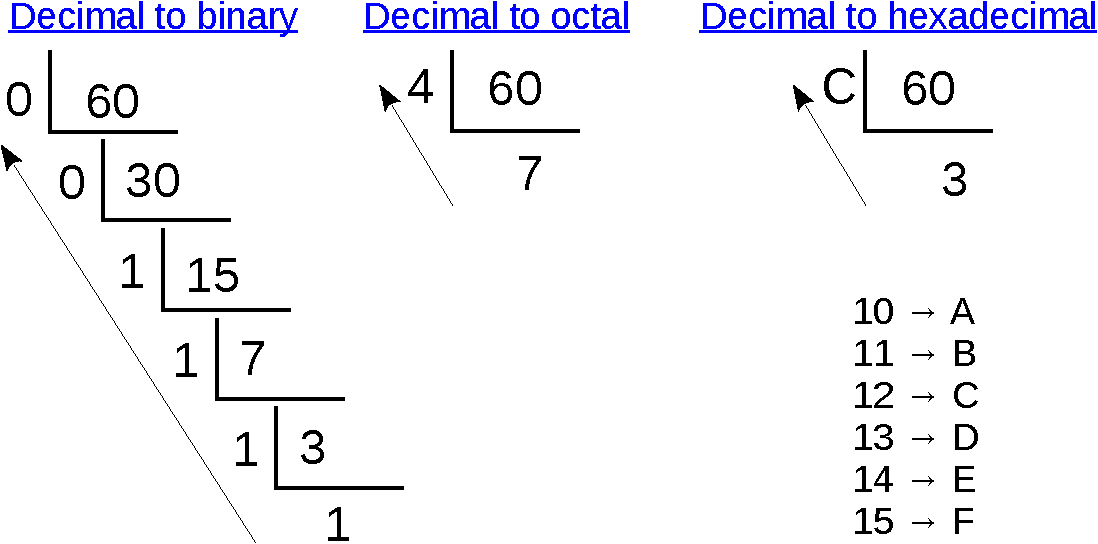
\includegraphics[width=0.75\linewidth]{figs/d2b_v2.pdf}
	\end{figure}
\end{frame}

\begin{frame}
\frametitle{Decimal to Binary, Octal and Hexadecimal (4)}
	\begin{figure}
		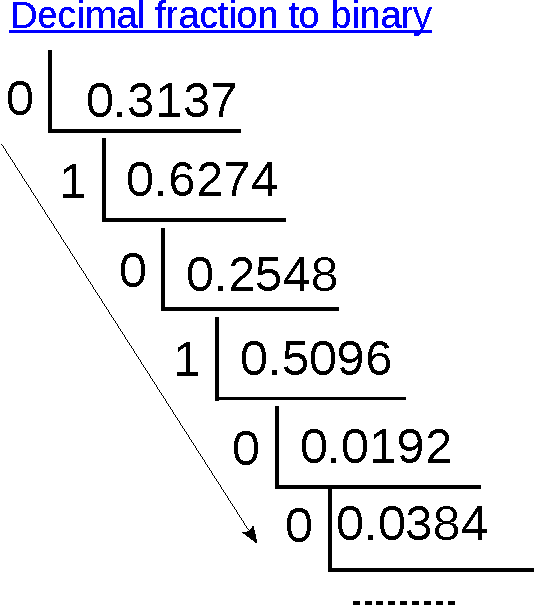
\includegraphics[width=0.45\linewidth]{figs/d2b1.pdf}
	\end{figure}
\begin{equation}
0{\times}2^{-1}+1{\times}2^{-2}+0{\times}2^{-3}+1{\times}2^{-4}=0.3125 \approx 0.3137 \nonumber
\end{equation}
\end{frame}

\begin{frame}
\frametitle{Binary, Octal and Hexadecimal to Decimal}
	\begin{itemize}
		\item {Binary code: $111100_{(2)}$}
		\item {Octal code: $74_{(8)}$}
		\item {Hexadecimal code: $3C_{(16)}$}
	\end{itemize}
	\begin{eqnarray}
		1\times2^5+1\times2^4+1\times2^3+1\times2^2+0\times2^1+0\times2^0=60 \nonumber \\
		7\times8^1+4\times8^0=60 \nonumber \\
		3\times16^1+12\times16^0=60 \nonumber
	\end{eqnarray}
\end{frame}


\begin{frame}
 \frametitle{Data in the memory (1)}
\begin{itemize}
	\item {Data in the memory is kept in binary form}
	\item {Given an integer \textbf{49}, its binary code is $110001_{(2)}$}
	\item {It is kept in following form}
\end{itemize}
\vspace{0.1in}
\begin{center}
\begin{tikzpicture}[font=\small,x=1.4cm]
		\begin{uncoverenv}<1->
			\node[red, below=.4em, right=0em, ] at (0,1.9) {0};
			\draw[blue] (0,1.6) -- (.5,1.6);
			\draw[blue] (.5,1.6) -- (.5,1.9);
			\draw[blue] (0,1.9) -- (.5,1.9);
			\draw[blue] (0,1.6) -- (0,1.9);
		
			\node[blue, below=.4em, right=0em, ] at (.5,1.9) {1};
			\draw[blue] (.5,1.6) -- (1,1.6);
			\draw[blue] (1,1.6) -- (1,1.9);
			\draw[blue] (.5,1.9) -- (1,1.9);
			\draw[blue] (.5,1.6) -- (.5,1.9);
			
			\node[blue, below=.4em, right=0em, ] at (1,1.9) {1};
			\draw[blue] (1,1.6) -- (1.5,1.6);
			\draw[blue] (1.5,1.6) -- (1.5,1.9);
			\draw[blue] (1,1.9) -- (1.5,1.9);
			\draw[blue] (1,1.6) -- (1,1.9);
		
			\node[blue, below=.4em, right=0em, ] at (1.5,1.9) {0};
			\draw[blue] (1.5,1.6) -- (2,1.6);
			\draw[blue] (2,1.6) -- (2,1.9);
			\draw[blue] (1.5,1.9) -- (2,1.9);
			\draw[blue] (1.5,1.6) -- (1.5,1.9);

			\node[blue, below=.4em, right=0em, ] at (2,1.9) {0};
			\draw[blue] (2,1.6) -- (2.5,1.6);
			\draw[blue] (2.5,1.6) -- (2.5,1.9);
			\draw[blue] (2,1.9) -- (2.5,1.9);
			\draw[blue] (2,1.6) -- (2,1.9);

			\node[blue, below=.4em, right=0em, ] at (2.5,1.9) {0};
			\draw[blue] (2.5,1.6) -- (3,1.6);
			\draw[blue] (3,1.6) -- (3,1.9);
			\draw[blue] (2.5,1.9) -- (3,1.9);
			\draw[blue] (2.5,1.6) -- (2.5,1.9);
			
			\node[blue, below=.4em, right=0em, ] at (3,1.9) {1};
			\draw[blue] (3,1.6) -- (3.5,1.6);
			\draw[blue] (3.5,1.6) -- (3.5,1.9);
			\draw[blue] (3,1.9) -- (3.5,1.9);
			\draw[blue] (3,1.6) -- (3,1.9);
		\end{uncoverenv}
	\end{tikzpicture}
\end{center}
\begin{itemize}
	\item {Given an integer \textbf{-49}, its binary code is \textcolor{red}{1}$110001_{(2)}$}
	\item {It is kept in following form}
\end{itemize}
\begin{center}
\begin{tikzpicture}[font=\small,x=1.4cm]
		\begin{uncoverenv}<1->
			\node[red, below=.4em, right=0em, ] at (0,1.9) {1};
			\draw[blue] (0,1.6) -- (.5,1.6);
			\draw[blue] (.5,1.6) -- (.5,1.9);
			\draw[blue] (0,1.9) -- (.5,1.9);
			\draw[blue] (0,1.6) -- (0,1.9);
		
			\node[blue, below=.4em, right=0em, ] at (.5,1.9) {1};
			\draw[blue] (.5,1.6) -- (1,1.6);
			\draw[blue] (1,1.6) -- (1,1.9);
			\draw[blue] (.5,1.9) -- (1,1.9);
			\draw[blue] (.5,1.6) -- (.5,1.9);
			
			\node[blue, below=.4em, right=0em, ] at (1,1.9) {1};
			\draw[blue] (1,1.6) -- (1.5,1.6);
			\draw[blue] (1.5,1.6) -- (1.5,1.9);
			\draw[blue] (1,1.9) -- (1.5,1.9);
			\draw[blue] (1,1.6) -- (1,1.9);
		
			\node[blue, below=.4em, right=0em, ] at (1.5,1.9) {0};
			\draw[blue] (1.5,1.6) -- (2,1.6);
			\draw[blue] (2,1.6) -- (2,1.9);
			\draw[blue] (1.5,1.9) -- (2,1.9);
			\draw[blue] (1.5,1.6) -- (1.5,1.9);

			\node[blue, below=.4em, right=0em, ] at (2,1.9) {0};
			\draw[blue] (2,1.6) -- (2.5,1.6);
			\draw[blue] (2.5,1.6) -- (2.5,1.9);
			\draw[blue] (2,1.9) -- (2.5,1.9);
			\draw[blue] (2,1.6) -- (2,1.9);

			\node[blue, below=.4em, right=0em, ] at (2.5,1.9) {0};
			\draw[blue] (2.5,1.6) -- (3,1.6);
			\draw[blue] (3,1.6) -- (3,1.9);
			\draw[blue] (2.5,1.9) -- (3,1.9);
			\draw[blue] (2.5,1.6) -- (2.5,1.9);
			
			\node[blue, below=.4em, right=0em, ] at (3,1.9) {1};
			\draw[blue] (3,1.6) -- (3.5,1.6);
			\draw[blue] (3.5,1.6) -- (3.5,1.9);
			\draw[blue] (3,1.9) -- (3.5,1.9);
			\draw[blue] (3,1.6) -- (3,1.9);
		\end{uncoverenv}
	\end{tikzpicture}
\end{center}
\begin{itemize}
	\item {The highest bit is reserved for sign}
	\item {This is true for \textbf{real} numbers later we will see}
	\item {We use 8 bits (1 byte), 2 bytes or more bytes to keep a number}
\end{itemize}

\begin{center}
\begin{tikzpicture}[font=\small,x=1.4cm]
		\begin{uncoverenv}<1->
			\node[red, below=.4em, right=0em, ] at (0,1.9) {1};
			\draw[blue] (0,1.6) -- (.5,1.6);
			\draw[blue] (.5,1.6) -- (.5,1.9);
			\draw[blue] (0,1.9) -- (.5,1.9);
			\draw[blue] (0,1.6) -- (0,1.9);

			\node[blue, below=.4em, right=0em, ] at (0.5,1.9) {0};
			\draw[blue] (.5,1.6) -- (1,1.6);
			\draw[blue] (1,1.6) -- (1,1.9);
			\draw[blue] (.5,1.9) -- (1,1.9);
			\draw[blue] (.5,1.6) -- (.5,1.9);
		
			\node[blue, below=.4em, right=0em, ] at (1.0,1.9) {1};
			\draw[blue] (1,1.6) -- (1.5,1.6);
			\draw[blue] (1.5,1.6) -- (1.5,1.9);
			\draw[blue] (1,1.9) -- (1.5,1.9);
			\draw[blue] (1,1.6) -- (1,1.9);
			
			\node[blue, below=.4em, right=0em, ] at (1.5,1.9) {1};
			\draw[blue] (1.5,1.6) -- (2,1.6);
			\draw[blue] (2,1.6) -- (2,1.9);
			\draw[blue] (1.5,1.9) -- (2,1.9);
			\draw[blue] (1.5,1.6) -- (1.5,1.9);
		
			\node[blue, below=.4em, right=0em, ] at (2.0,1.9) {0};
			\draw[blue] (2,1.6) -- (2.5,1.6);
			\draw[blue] (2.5,1.6) -- (2.5,1.9);
			\draw[blue] (2,1.9) -- (2.5,1.9);
			\draw[blue] (2,1.6) -- (2,1.9);

			\node[blue, below=.4em, right=0em, ] at (2.5,1.9) {0};
			\draw[blue] (2.5,1.6) -- (3,1.6);
			\draw[blue] (3,1.6) -- (3,1.9);
			\draw[blue] (2.5,1.9) -- (3,1.9);
			\draw[blue] (2.5,1.6) -- (2.5,1.9);

			\node[blue, below=.4em, right=0em, ] at (3.0,1.9) {0};
			\draw[blue] (3,1.6) -- (3.5,1.6);
			\draw[blue] (3.5,1.6) -- (3.5,1.9);
			\draw[blue] (3,1.9) -- (3.5,1.9);
			\draw[blue] (3,1.6) -- (3,1.9);
			
			\node[blue, below=.4em, right=0em, ] at (3.5,1.9) {1};
			\draw[blue] (3.5,1.6) -- (4,1.6);
			\draw[blue] (4,1.6) -- (4,1.9);
			\draw[blue] (3.5,1.9) -- (4,1.9);
			\draw[blue] (3.5,1.6) -- (3.5,1.9);
		\end{uncoverenv}
	\end{tikzpicture}
\end{center}

\end{frame}

\begin{frame}
 \frametitle{Data in the memory (2)}
\begin{itemize}
	\item {Data in the memory is kept in binary form}
	\item {Given we have several numbers to be kept}
	\item {They are kept one after another (assume we use 1 byte for one number)}
\end{itemize}
\begin{center}
\begin{tikzpicture}[font=\small,x=1.4cm]
		\begin{uncoverenv}<1->
			\node[black, below=.4em, right=0em, ] at (-0.8,1.9) {0000};
			\node[red, below=.4em, right=0em, ] at (0,1.9) {1};
			\draw[blue] (0,1.6) -- (.5,1.6);
			\draw[blue] (.5,1.6) -- (.5,1.9);
			\draw[blue] (0,1.9) -- (.5,1.9);
			\draw[blue] (0,1.6) -- (0,1.9);

			\node[black, below=.4em, right=0em, ] at (-0.8,1.5) {0001};
			\node[red, below=.4em, right=0em, ] at (0,1.5) {0};
			\draw[blue] (0,1.2) -- (.5,1.2);
			\draw[blue] (.5,1.2) -- (.5,1.5);
			\draw[blue] (0,1.5) -- (.5,1.5);
			\draw[blue] (0,1.2) -- (0,1.5);

			\node[black, below=.4em, right=0em, ] at (-0.8,1.1) {0002};
			\node[black, below=.4em, right=0em, ] at (-0.8,0.7) {0003};
			\node[red, below=.4em, right=0em, ] at (0,1.1) {0};
			\draw[blue] (0,0.8) -- (.5,0.8);
			\draw[blue] (.5,0.8) -- (.5,1.1);
			\draw[blue] (0,1.1) -- (.5,1.1);
			\draw[blue] (0,0.8) -- (0,1.1);
			%%1st bit

			\node[blue, below=.4em, right=0em, ] at (0.5,0.7) {.};
			\node[blue, below=.4em, right=0em, ] at (0.5,1.9) {0};
			\draw[blue] (.5,1.6) -- (1,1.6);
			\draw[blue] (1,1.6) -- (1,1.9);
			\draw[blue] (.5,1.9) -- (1,1.9);
			\draw[blue] (.5,1.6) -- (.5,1.9);

			\node[blue, below=.4em, right=0em, ] at (0.5,1.5) {0};
			\draw[blue] (.5,1.2) -- (1,1.2);
			\draw[blue] (1,1.2) -- (1,1.5);
			\draw[blue] (.5,1.5) -- (1,1.5);
			\draw[blue] (.5,1.2) -- (.5,1.5);

			\node[blue, below=.4em, right=0em, ] at (0.5,1.1) {1};
			\draw[blue] (.5,0.8) -- (1,0.8);
			\draw[blue] (1,0.8) -- (1,1.1);
			\draw[blue] (.5,1.1) -- (1,1.1);
			\draw[blue] (.5,0.8) -- (.5,1.1);
			%%2nd bit

			\node[blue, below=.4em, right=0em, ] at (1.0,0.7) {.};		
			\node[blue, below=.4em, right=0em, ] at (1.0,1.9) {1};
			\draw[blue] (1,1.6) -- (1.5,1.6);
			\draw[blue] (1.5,1.6) -- (1.5,1.9);
			\draw[blue] (1,1.9) -- (1.5,1.9);
			\draw[blue] (1,1.6) -- (1,1.9);

			\node[blue, below=.4em, right=0em, ] at (1.0,1.5) {1};
			\draw[blue] (1,1.2) -- (1.5,1.2);
			\draw[blue] (1.5,1.2) -- (1.5,1.5);
			\draw[blue] (1,1.5) -- (1.5,1.5);
			\draw[blue] (1,1.2) -- (1,1.5);
		
			\node[blue, below=.4em, right=0em, ] at (1.0,1.1) {0};
			\draw[blue] (1,0.8) -- (1.5,0.8);
			\draw[blue] (1.5,0.8) -- (1.5,1.1);
			\draw[blue] (1,1.1) -- (1.5,1.1);
			\draw[blue] (1,0.8) -- (1,1.1);
			%%3rd
			
			\node[blue, below=.4em, right=0em, ] at (1.5,1.9) {1};
			\draw[blue] (1.5,1.6) -- (2,1.6);
			\draw[blue] (2,1.6) -- (2,1.9);
			\draw[blue] (1.5,1.9) -- (2,1.9);
			\draw[blue] (1.5,1.6) -- (1.5,1.9);

			\node[blue, below=.4em, right=0em, ] at (1.5,1.5) {1};
			\draw[blue] (1.5,1.2) -- (2,1.2);
			\draw[blue] (2,1.2) -- (2,1.5);
			\draw[blue] (1.5,1.5) -- (2,1.5);
			\draw[blue] (1.5,1.2) -- (1.5,1.5);
		
			\node[blue, below=.4em, right=0em, ] at (1.5,1.1) {1};
			\draw[blue] (1.5,0.8) -- (2,0.8);
			\draw[blue] (2,0.8) -- (2,1.1);
			\draw[blue] (1.5,1.1) -- (2,1.1);
			\draw[blue] (1.5,0.8) -- (1.5,1.1);
			%%4th
		
			\node[blue, below=.4em, right=0em, ] at (2.0,1.9) {0};
			\draw[blue] (2,1.6) -- (2.5,1.6);
			\draw[blue] (2.5,1.6) -- (2.5,1.9);
			\draw[blue] (2,1.9) -- (2.5,1.9);
			\draw[blue] (2,1.6) -- (2,1.9);

			\node[blue, below=.4em, right=0em, ] at (2.0,1.5) {0};
			\draw[blue] (2,1.2) -- (2.5,1.2);
			\draw[blue] (2.5,1.2) -- (2.5,1.5);
			\draw[blue] (2,1.5) -- (2.5,1.5);
			\draw[blue] (2,1.2) -- (2,1.5);
			
			\node[blue, below=.4em, right=0em, ] at (2.0,1.1) {1};
			\draw[blue] (2,0.8) -- (2.5,0.8);
			\draw[blue] (2.5,0.8) -- (2.5,1.1);
			\draw[blue] (2,1.1) -- (2.5,1.1);
			\draw[blue] (2,0.8) -- (2,1.1);
			%%5th

			\node[blue, below=.4em, right=0em, ] at (2.5,1.9) {0};
			\draw[blue] (2.5,1.6) -- (3,1.6);
			\draw[blue] (3,1.6) -- (3,1.9);
			\draw[blue] (2.5,1.9) -- (3,1.9);
			\draw[blue] (2.5,1.6) -- (2.5,1.9);
			
			\node[blue, below=.4em, right=0em, ] at (2.5,1.5) {0};
			\draw[blue] (2.5,1.2) -- (3,1.2);
			\draw[blue] (3,1.2) -- (3,1.5);
			\draw[blue] (2.5,1.5) -- (3,1.5);
			\draw[blue] (2.5,1.2) -- (2.5,1.5);
			
			\node[blue, below=.4em, right=0em, ] at (2.5,1.1) {1};
			\draw[blue] (2.5,0.8) -- (3,0.8);
			\draw[blue] (3,0.8) -- (3,1.1);
			\draw[blue] (2.5,1.1) -- (3,1.1);
			\draw[blue] (2.5,0.8) -- (2.5,1.1);
			%%6th

			\node[blue, below=.4em, right=0em, ] at (3.0,1.9) {0};
			\draw[blue] (3,1.6) -- (3.5,1.6);
			\draw[blue] (3.5,1.6) -- (3.5,1.9);
			\draw[blue] (3,1.9) -- (3.5,1.9);
			\draw[blue] (3,1.6) -- (3,1.9);

			\node[blue, below=.4em, right=0em, ] at (3.0,1.5) {1};
			\draw[blue] (3,1.2) -- (3.5,1.2);
			\draw[blue] (3.5,1.2) -- (3.5,1.5);
			\draw[blue] (3,1.5) -- (3.5,1.5);
			\draw[blue] (3,1.2) -- (3,1.5);

			\node[blue, below=.4em, right=0em, ] at (3.0,1.1) {0};
			\draw[blue] (3,0.8) -- (3.5,0.8);
			\draw[blue] (3.5,0.8) -- (3.5,1.1);
			\draw[blue] (3,1.1) -- (3.5,1.1);
			\draw[blue] (3,0.8) -- (3,1.1);
			%%7th
			
			\node[blue, below=.4em, right=0em, ] at (3.5,1.9) {1};
			\draw[blue] (3.5,1.6) -- (4,1.6);
			\draw[blue] (4,1.6) -- (4,1.9);
			\draw[blue] (3.5,1.9) -- (4,1.9);
			\draw[blue] (3.5,1.6) -- (3.5,1.9);

			\node[blue, below=.4em, right=0em, ] at (3.5,1.5) {1};
			\draw[blue] (3.5,1.2) -- (4,1.2);
			\draw[blue] (4,1.2) -- (4,1.5);
			\draw[blue] (3.5,1.5) -- (4,1.5);
			\draw[blue] (3.5,1.2) -- (3.5,1.5);
			
			\node[blue, below=.4em, right=0em, ] at (3.5,1.1) {1};
			\draw[blue] (3.5,0.8) -- (4,0.8);
			\draw[blue] (4,0.8) -- (4,1.1);
			\draw[blue] (3.5,1.1) -- (4,1.1);
			\draw[blue] (3.5,0.8) -- (3.5,1.1);
		\end{uncoverenv}
	\end{tikzpicture}
\end{center}

\end{frame}

\begin{frame}
	\frametitle{Data in the memory (3)}
	\begin{itemize}
		\item {Now, think about an important issue}
		\item {Given 1 byte, how many different numbers we can represent}
		\item {Assuming no sign bit}
	\end{itemize}
	\begin{figure}
		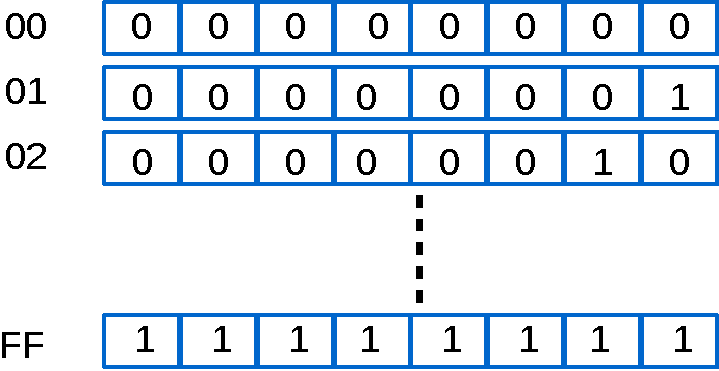
\includegraphics[width=0.55\linewidth]{figs/byte.pdf}
	\end{figure}
	\begin{itemize}
		\item {With 1 byte, there are \textbf{$2^8=256$} numbers}
		\item {Since our memory are limited, we can only represent a limited range of numbers}
	\end{itemize}
\end{frame}


\begin{frame}
	\frametitle{Data in the memory (4)}
	\begin{itemize}
		\item {Now, think about how many different numbers we have if one bit is reserved for sign}
		\item {????}
	\end{itemize}
\end{frame}

\begin{frame}
	\frametitle{Data in the memory (5)}
	\begin{itemize}
		\item {Now, think about how many different numbers we have if one bit is reserved for sign}
		\item {$2{\times}2^7-1=255$}
		\item {Only 127 positive numbers (1 $\sim$ 127)}
		\item {127 negatives (-1 $\sim$ -127)}
	\end{itemize}
	\begin{itemize}
		\item {Some numbers can only be approximately represented by binary code}
		\item {For example, \textbf{3.3137}}
		\item {$11.0101_{(2)}$}
	\end{itemize}
\end{frame}

\begin{frame}
	\frametitle{One's complement and Two's Complement}
\begin{table}
\begin{center}
\begin{tabular}{|c|c|c|c|}
\hline
Original & bits & One's Complement & Two's Complement \\ \hline
23   & \textcolor{red}{0}0010111 & \textcolor{red}{0}0010111 & \textcolor{red}{0}0010111 \\ \hline 
-23   & \textcolor{red}{1}0010111 & \textcolor{red}{1}1101000 & \textcolor{red}{1}1101001 \\ \hline \hline
33   & \textcolor{red}{0}0100001 & \textcolor{red}{0}0100001 & \textcolor{red}{0}0100001 \\ \hline
-33   & \textcolor{red}{1}0100001 & \textcolor{red}{1}1011110 & \textcolor{red}{1}1011111 \\ \hline  
\end{tabular}
\end{center}
\end{table}
\begin{itemize}
	\item {One's complement and two's complement of positive numbers are the same as original code}
	\item {For negative number, we do not inverse its sign bit}
	\item {Why we do so??}
	\begin{itemize}
		\item {It is very convenient when we do substraction}
		\item {Substraction is converted to add operation}
	\end{itemize}
	\item {Now please work out one's complement and two's complement of \textbf{-17}}
\end{itemize}
\end{frame}